\documentclass{article}
\usepackage{tikz}
\usepackage{pgfplots}
\usepackage{textcomp}
\usepackage{array}
\usepackage{tabu}
\usepackage{numprint}
\begin{document}
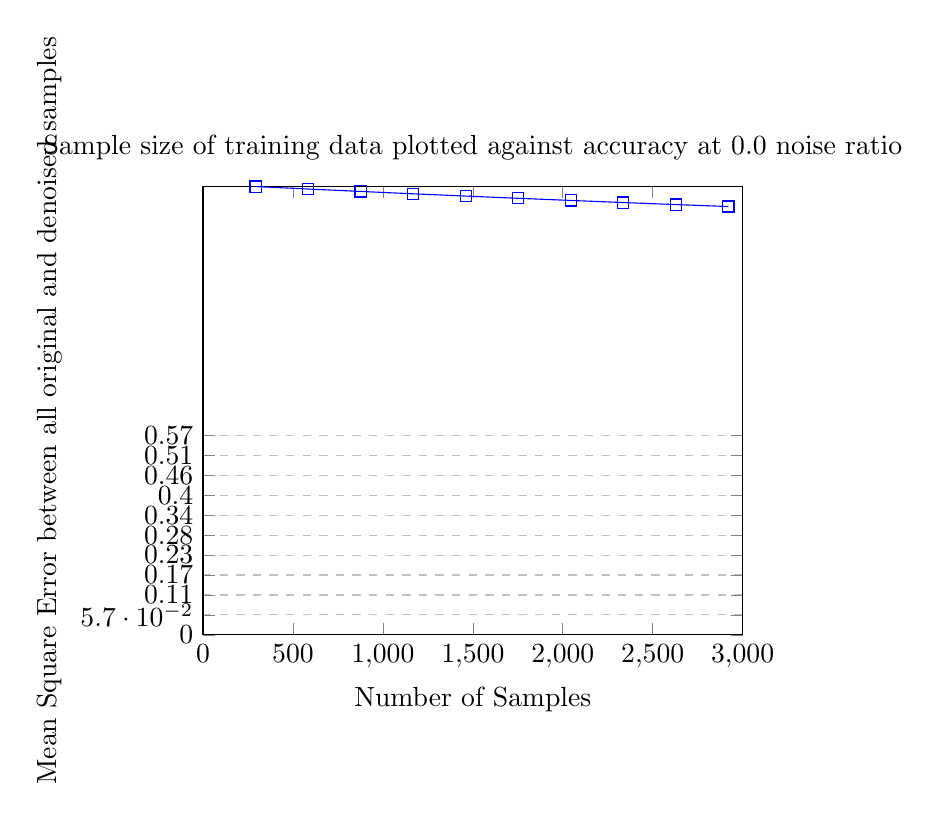
\begin{tikzpicture}
\begin{axis}[
title={Sample size of training data plotted against accuracy at 0.0 noise ratio},
xlabel={Number of Samples},
ylabel={Mean Square Error between all original and denoised samples},
xmin=0, xmax=3000,
ymin=0, ymax=1.2800689509826504,
xtick={0,500,1000,1500,2000,2500,3000},
ytick={0,0.05697317205321739,0.11394634410643478,0.17091951615965217,0.22789268821286957,0.28486586026608696,0.34183903231930435,0.39881220437252174,0.45578537642573913,0.5127585484789565,0.5697317205321739},
legend pos=north west,
ymajorgrids=true,
grid style=dashed,
]

\addplot[
color=blue,
mark=square,
]
coordinates {

(292, 1.2800689509826504)
(584, 1.2730905881325858)
(876, 1.2661602065517217)
(1168, 1.2594348782340052)
(1460, 1.252921269619059)
(1752, 1.2465698739643452)
(2044, 1.2404369443263132)
(2336, 1.234460650291608)
(2628, 1.2286727424691126)
(2921, 1.223095778929433)
    };
\end{axis}
\end{tikzpicture}

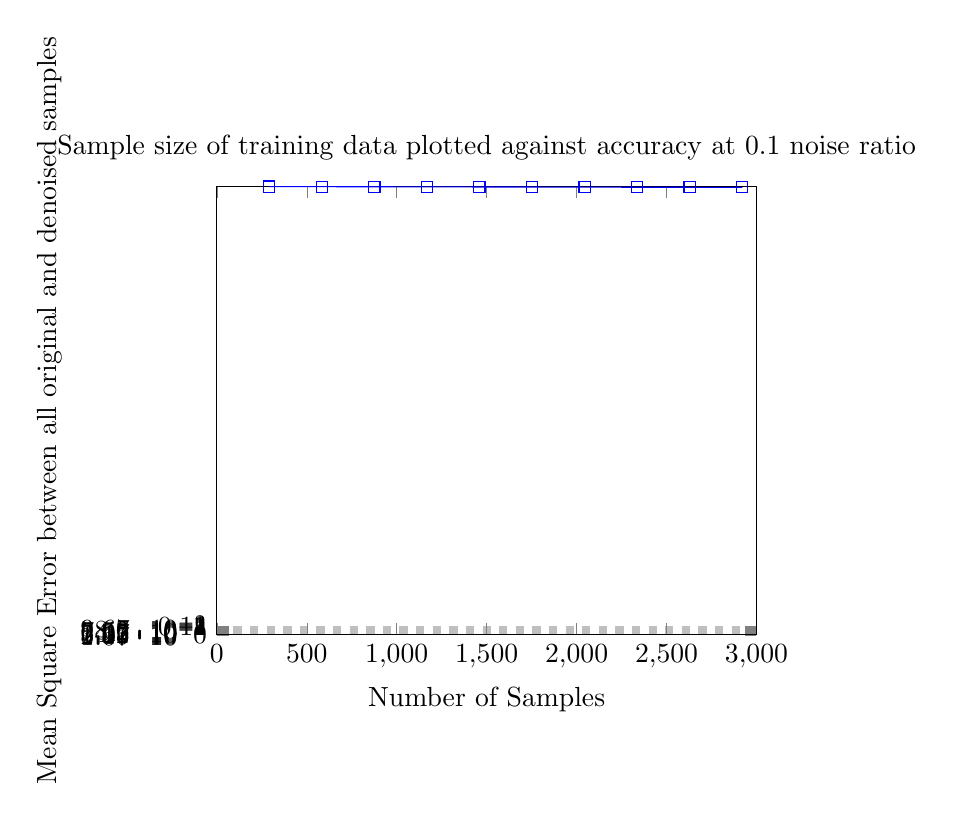
\begin{tikzpicture}
\begin{axis}[
title={Sample size of training data plotted against accuracy at 0.1 noise ratio},
xlabel={Number of Samples},
ylabel={Mean Square Error between all original and denoised samples},
xmin=0, xmax=3000,
ymin=0, ymax=5.886330744004356,
xtick={0,500,1000,1500,2000,2500,3000},
ytick={0,0.010744421059547982,0.021488842119095963,0.032233263178643945,0.04297768423819193,0.05372210529773991,0.06446652635728789,0.07521094741683587,0.08595536847638385,0.09669978953593183,0.10744421059547982},
legend pos=north west,
ymajorgrids=true,
grid style=dashed,
]

\addplot[
color=blue,
mark=square,
]
coordinates {

(292, 5.886330744004356)
(584, 5.884970812888446)
(876, 5.88366300358988)
(1168, 5.8823930090320555)
(1460, 5.88117721372258)
(1752, 5.880009605442368)
(2044, 5.878845408609814)
(2336, 5.8777213086894005)
(2628, 5.876642704396269)
(2921, 5.875586322944808)
    };
\end{axis}
\end{tikzpicture}


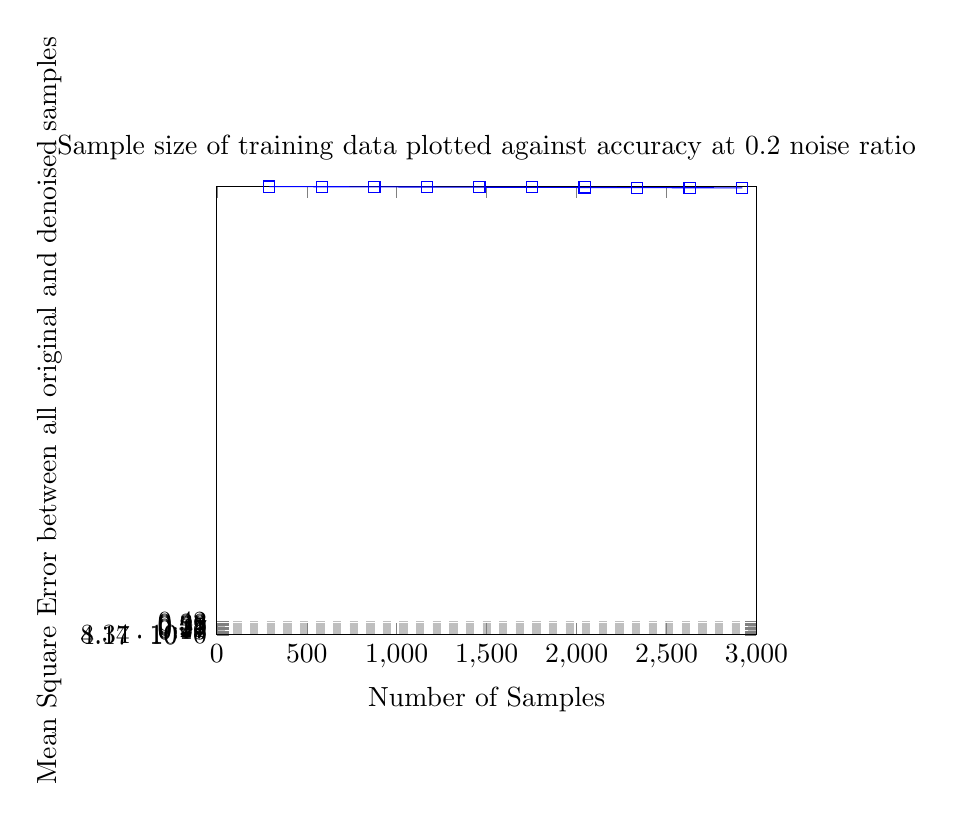
\begin{tikzpicture}
\begin{axis}[
title={Sample size of training data plotted against accuracy at 0.2 noise ratio},
xlabel={Number of Samples},
ylabel={Mean Square Error between all original and denoised samples},
xmin=0, xmax=3000,
ymin=0, ymax=14.251296352133465,
xtick={0,500,1000,1500,2000,2500,3000},
ytick={0,0.04168180525562981,0.08336361051125962,0.12504541576688943,0.16672722102251925,0.20840902627814906,0.25009083153377887,0.2917726367894087,0.3334544420450385,0.3751362473006683,0.4168180525562981},
legend pos=north west,
ymajorgrids=true,
grid style=dashed,
]

\addplot[
color=blue,
mark=square,
]
coordinates {

(292, 14.251296352133465)
(584, 14.246251863285348)
(876, 14.241324020467781)
(1168, 14.23647321352)
(1460, 14.231724170212507)
(1752, 14.227072927232085)
(2044, 14.222542433962081)
(2336, 14.218113382389486)
(2628, 14.213822514427973)
(2921, 14.209614546877836)
    };
\end{axis}
\end{tikzpicture}


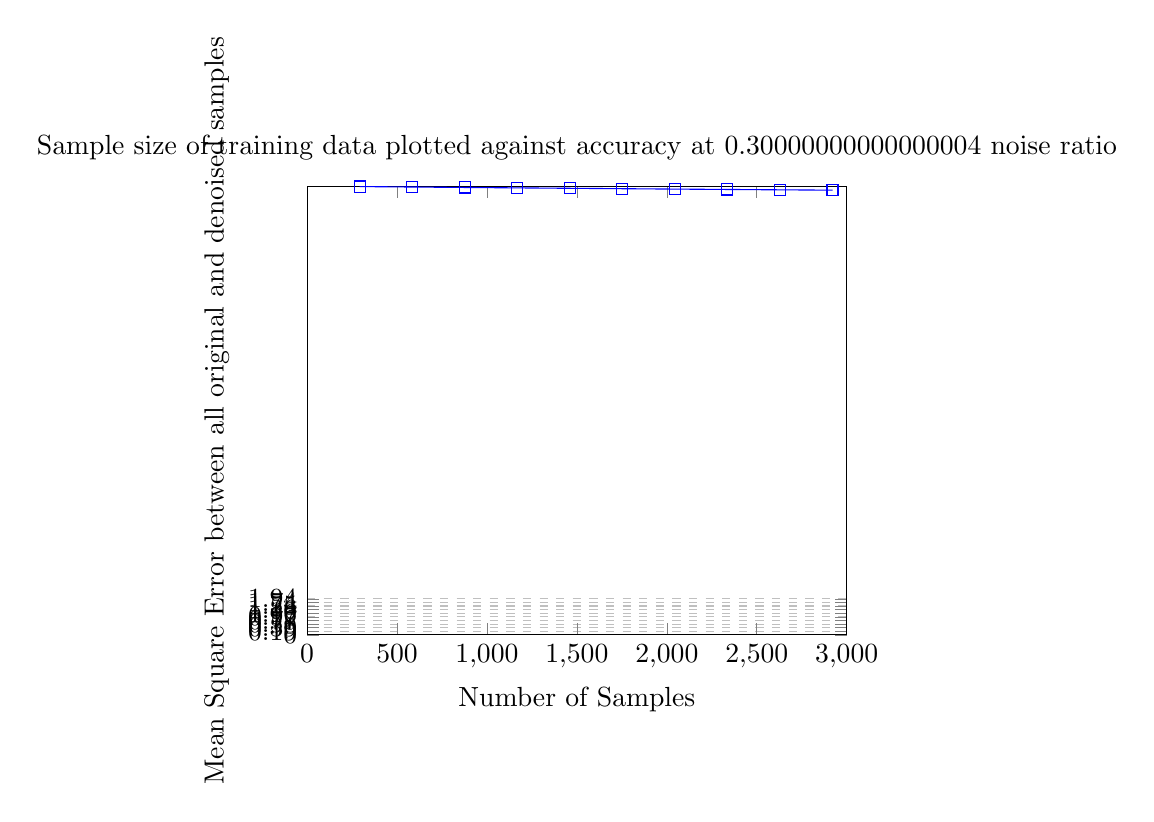
\begin{tikzpicture}
\begin{axis}[
title={Sample size of training data plotted against accuracy at 0.30000000000000004 noise ratio},
xlabel={Number of Samples},
ylabel={Mean Square Error between all original and denoised samples},
xmin=0, xmax=3000,
ymin=0, ymax=24.071912267044898,
xtick={0,500,1000,1500,2000,2500,3000},
ytick={0,0.1936285895995944,0.3872571791991888,0.5808857687987832,0.7745143583983776,0.968142947997972,1.1617715375975664,1.3554001271971607,1.5490287167967551,1.7426573063963495,1.936285895995944},
legend pos=north west,
ymajorgrids=true,
grid style=dashed,
]

\addplot[
color=blue,
mark=square,
]
coordinates {

(292, 24.071912267044898)
(584, 24.047772466468878)
(876, 24.0241341208634)
(1168, 24.00118091540419)
(1460, 23.97887436944461)
(1752, 23.957246247859807)
(2044, 23.936354235764487)
(2336, 23.916261054738925)
(2628, 23.896899545638902)
(2921, 23.878283677445303)
    };
\end{axis}
\end{tikzpicture}


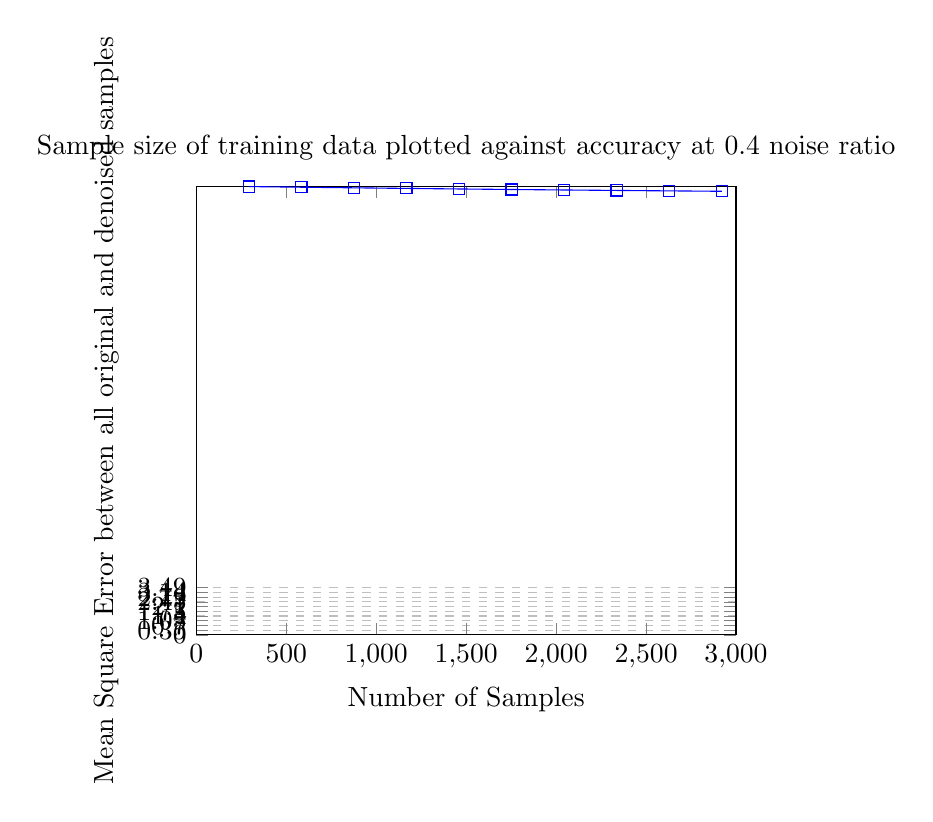
\begin{tikzpicture}
\begin{axis}[
title={Sample size of training data plotted against accuracy at 0.4 noise ratio},
xlabel={Number of Samples},
ylabel={Mean Square Error between all original and denoised samples},
xmin=0, xmax=3000,
ymin=0, ymax=33.154912822510575,
xtick={0,500,1000,1500,2000,2500,3000},
ytick={0,0.34928760131370495,0.6985752026274099,1.0478628039411149,1.3971504052548198,1.7464380065685248,2.0957256078822297,2.4450132091959347,2.7943008105096396,3.1435884118233446,3.4928760131370495},
legend pos=north west,
ymajorgrids=true,
grid style=dashed,
]

\addplot[
color=blue,
mark=square,
]
coordinates {

(292, 33.154912822510575)
(584, 33.10703288414358)
(876, 33.06146159357696)
(1168, 33.018208592287166)
(1460, 32.97720983641984)
(1752, 32.93861497162867)
(2044, 32.902305578221785)
(2336, 32.8680511121948)
(2628, 32.835847787840855)
(2921, 32.80562522119687)
    };
\end{axis}
\end{tikzpicture}


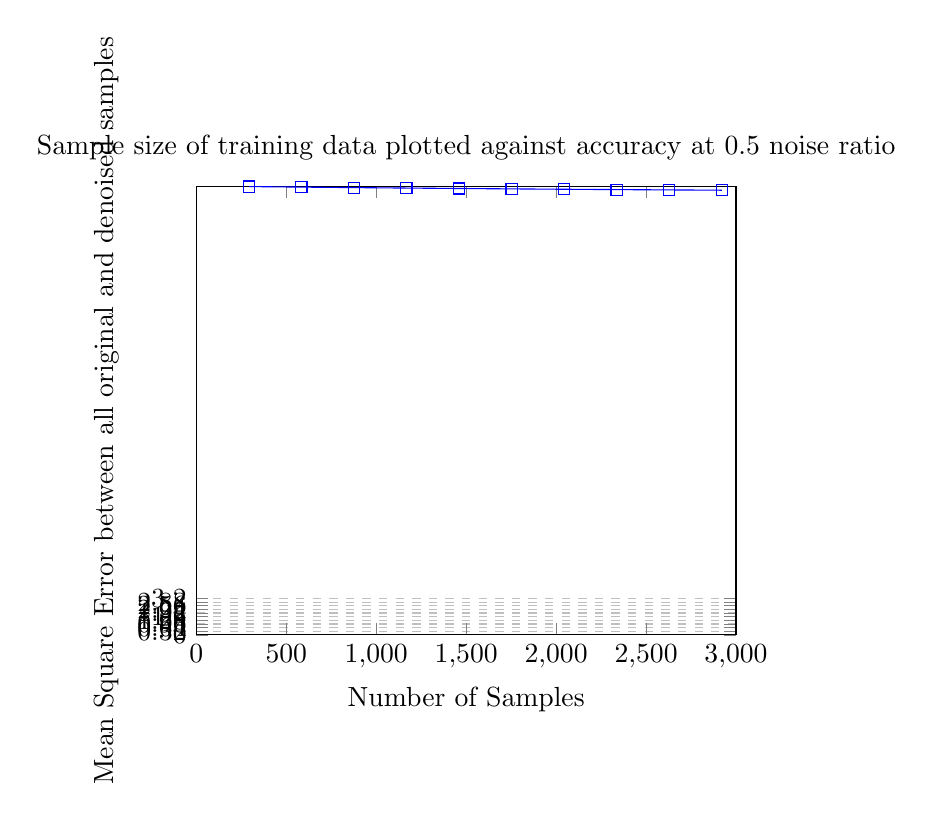
\begin{tikzpicture}
\begin{axis}[
title={Sample size of training data plotted against accuracy at 0.5 noise ratio},
xlabel={Number of Samples},
ylabel={Mean Square Error between all original and denoised samples},
xmin=0, xmax=3000,
ymin=0, ymax=39.422025892077755,
xtick={0,500,1000,1500,2000,2500,3000},
ytick={0,0.320336731415253,0.640673462830506,0.961010194245759,1.281346925661012,1.601683657076265,1.922020388491518,2.242357119906771,2.562693851322024,2.883030582737277,3.20336731415253},
legend pos=north west,
ymajorgrids=true,
grid style=dashed,
]

\addplot[
color=blue,
mark=square,
]
coordinates {

(292, 39.422025892077755)
(584, 39.37476664249158)
(876, 39.33094490121786)
(1168, 39.29032960107698)
(1460, 39.252640166626186)
(1752, 39.217820724657265)
(2044, 39.18542303505114)
(2336, 39.15542758731611)
(2628, 39.127614112805084)
(2921, 39.1016891606625)
    };
\end{axis}
\end{tikzpicture}


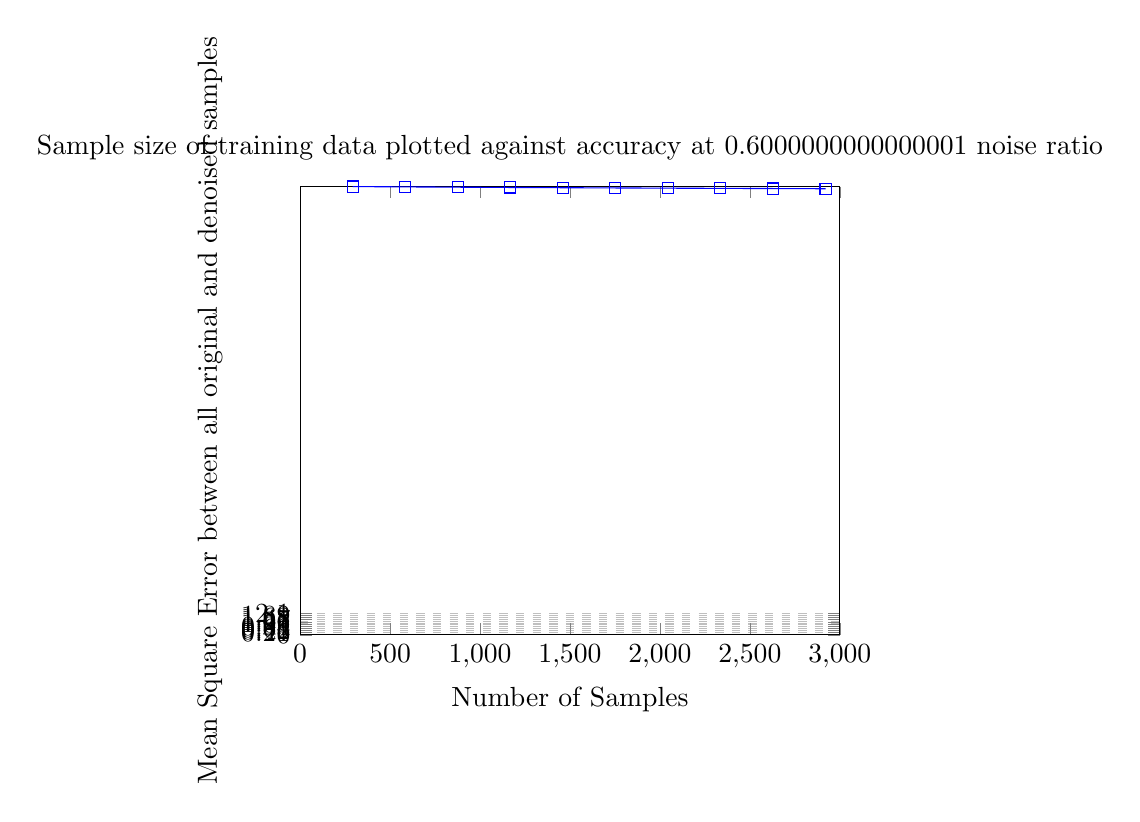
\begin{tikzpicture}
\begin{axis}[
title={Sample size of training data plotted against accuracy at 0.6000000000000001 noise ratio},
xlabel={Number of Samples},
ylabel={Mean Square Error between all original and denoised samples},
xmin=0, xmax=3000,
ymin=0, ymax=43.363946300400826,
xtick={0,500,1000,1500,2000,2500,3000},
ytick={0,0.20967197950237448,0.41934395900474897,0.6290159385071235,0.8386879180094979,1.0483598975118724,1.258031877014247,1.4677038565166214,1.6773758360189959,1.8870478155213704,2.096719795023745},
legend pos=north west,
ymajorgrids=true,
grid style=dashed,
]

\addplot[
color=blue,
mark=square,
]
coordinates {

(292, 43.363946300400826)
(584, 43.3328448421986)
(876, 43.304120453762245)
(1168, 43.277566190505524)
(1460, 43.253014308955215)
(1752, 43.230281095600965)
(2044, 43.20916440416408)
(2336, 43.189543872239675)
(2628, 43.17131697330742)
(2921, 43.15427432089845)
    };
\end{axis}
\end{tikzpicture}



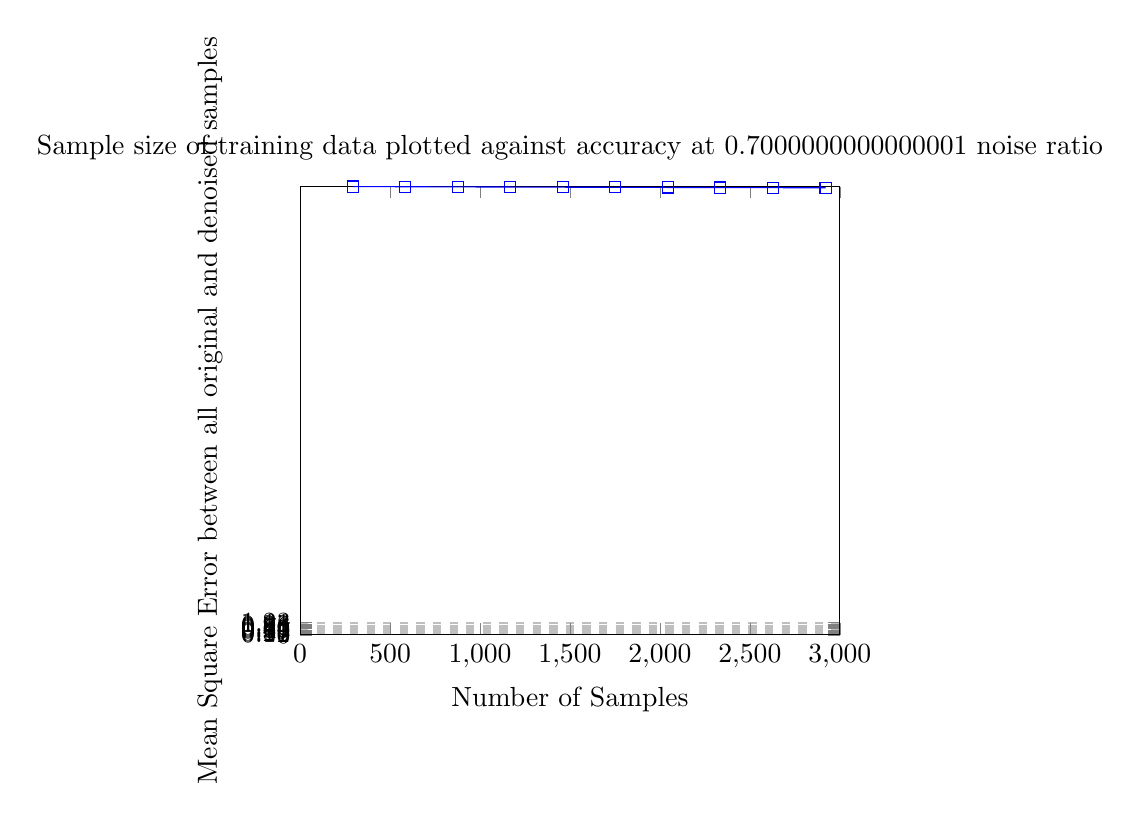
\begin{tikzpicture}
\begin{axis}[
title={Sample size of training data plotted against accuracy at 0.7000000000000001 noise ratio},
xlabel={Number of Samples},
ylabel={Mean Square Error between all original and denoised samples},
xmin=0, xmax=3000,
ymin=0, ymax=44.92530398952833,
xtick={0,500,1000,1500,2000,2500,3000},
ytick={0,0.12284745519638562,0.24569491039277125,0.3685423655891569,0.4913898207855425,0.6142372759819281,0.7370847311783137,0.8599321863746994,0.982779641571085,1.1056270967674706,1.2284745519638562},
legend pos=north west,
ymajorgrids=true,
grid style=dashed,
]

\addplot[
color=blue,
mark=square,
]
coordinates {

(292, 44.92530398952833)
(584, 44.90770200068133)
(876, 44.89130330171674)
(1168, 44.875998094667445)
(1460, 44.861698044811696)
(1752, 44.84830049809103)
(2044, 44.83576165136282)
(2336, 44.82399646694337)
(2628, 44.81289926179125)
(2921, 44.802456534331945)
    };
\end{axis}
\end{tikzpicture}


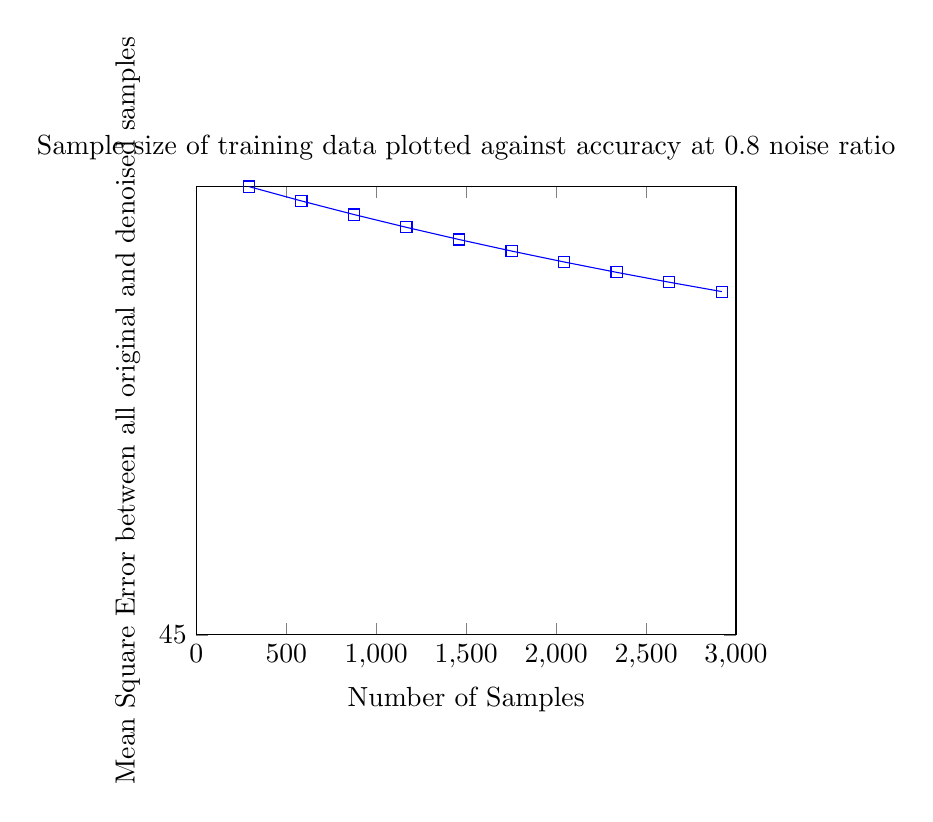
\begin{tikzpicture}
\begin{axis}[
title={Sample size of training data plotted against accuracy at 0.8 noise ratio},
xlabel={Number of Samples},
ylabel={Mean Square Error between all original and denoised samples},
xmin=0, xmax=3000,
ymin=45, ymax=45.302047236494445,
xtick={0,500,1000,1500,2000,2500,3000},
ytick={45},
legend pos=north west,
ymajorgrids=true,
grid style=dashed,
]

\addplot[
color=blue,
mark=square,
]
coordinates {

(292, 45.302047236494445)
(584, 45.29235450573169)
(876, 45.2832030967193)
(1168, 45.27456688970279)
(1460, 45.26638580855972)
(1752, 45.25860471705104)
(2044, 45.25125429360064)
(2336, 45.244258975250276)
(2628, 45.237612361105555)
(2921, 45.23128408399811)
    };
\end{axis}
\end{tikzpicture}


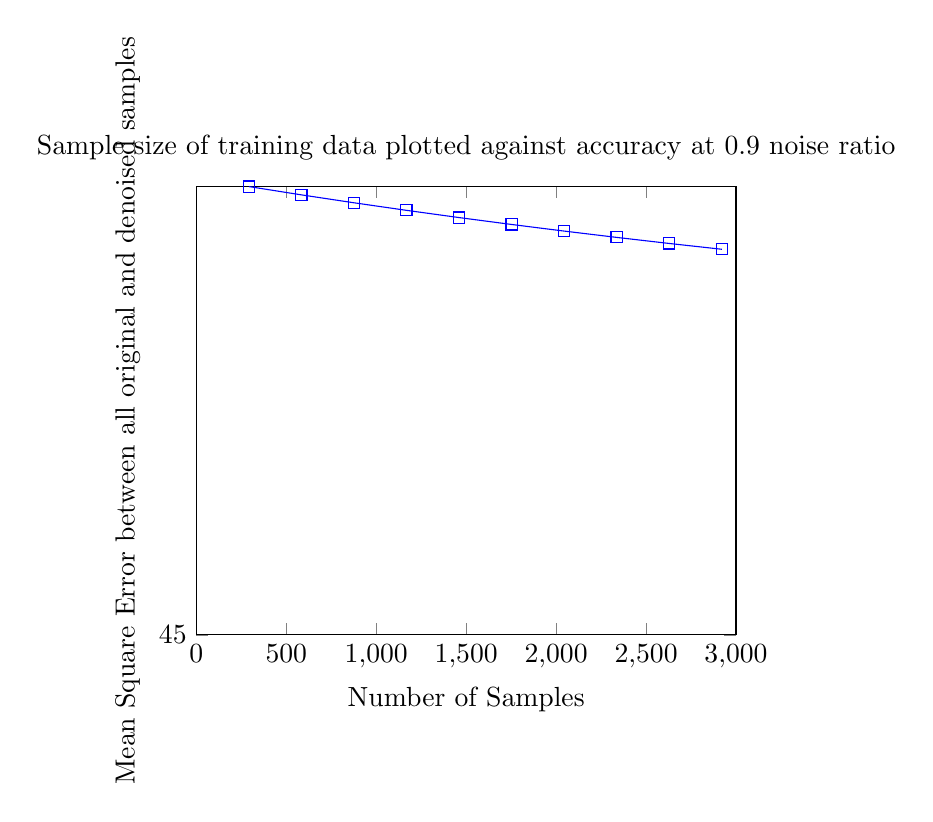
\begin{tikzpicture}
\begin{axis}[
title={Sample size of training data plotted against accuracy at 0.9 noise ratio},
xlabel={Number of Samples},
ylabel={Mean Square Error between all original and denoised samples},
xmin=0, xmax=3000,
ymin=45, ymax=45.331248975937825,
xtick={0,500,1000,1500,2000,2500,3000},
ytick={45},
legend pos=north west,
ymajorgrids=true,
grid style=dashed,
]

\addplot[
color=blue,
mark=square,
]
coordinates {

(292, 45.331248975937825)
(584, 45.32511124714941)
(876, 45.31926596185741)
(1168, 45.31367761690851)
(1460, 45.308340265049985)
(1752, 45.30325015027416)
(2044, 45.298364974054415)
(2336, 45.29369513569068)
(2628, 45.28921736901771)
(2921, 45.28492093077169)
    };
\end{axis}
\end{tikzpicture}




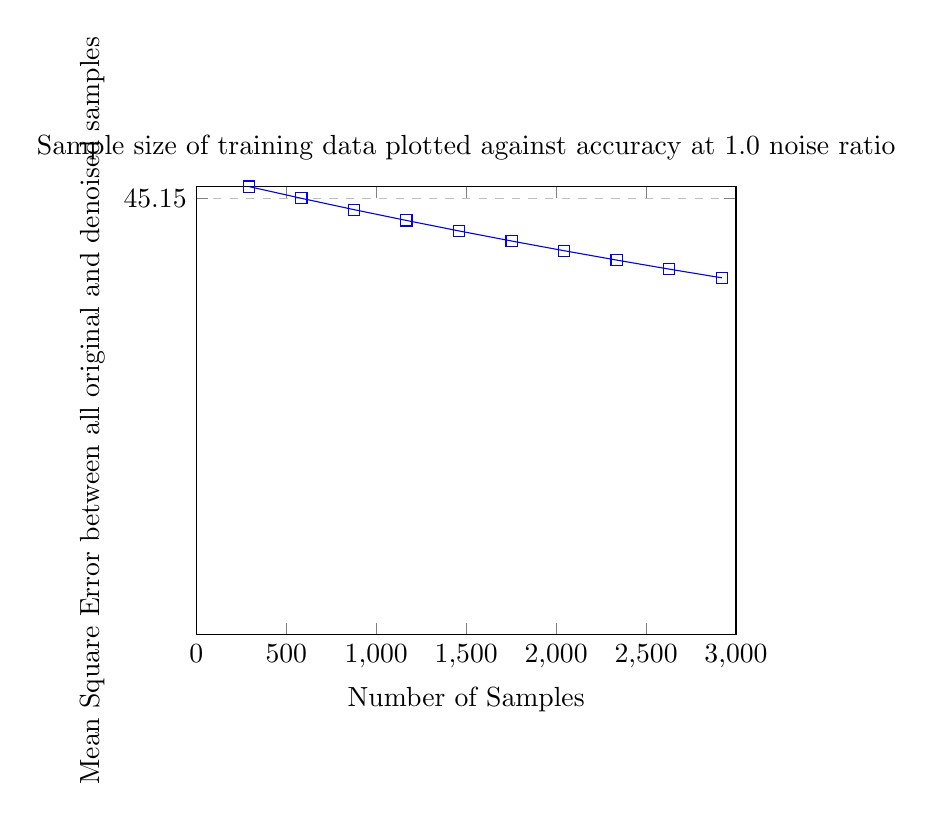
\begin{tikzpicture}
\begin{axis}[
title={Sample size of training data plotted against accuracy at 1.0 noise ratio},
xlabel={Number of Samples},
ylabel={Mean Square Error between all original and denoised samples},
xmin=0, xmax=3000,
ymin=45, ymax=45.15334736103961,
xtick={0,500,1000,1500,2000,2500,3000},
ytick={45.149327744025854},
legend pos=north west,
ymajorgrids=true,
grid style=dashed,
]

\addplot[
color=blue,
mark=square,
]
coordinates {

(292, 45.15334736103961)
(584, 45.149327744025854)
(876, 45.14545703337025)
(1168, 45.14174835329261)
(1460, 45.138169225731474)
(1752, 45.134726060469276)
(2044, 45.131407507967836)
(2336, 45.1282031322717)
(2628, 45.125111494800834)
(2921, 45.122133955066076)
    };
\end{axis}
\end{tikzpicture}


\end{document}